\section*{DAMPING FROM FREE ROLL DECAY SIGNALS}\label{sec:damping_free_roll_decay}

The mathematical model of a ship's free roll decay can be described in terms of damping, stiffness and inertia coefficients. The roll motion response of the free roll decay can be expressed in a general form according to \citep{7505983/FB64RGPF}

\begin{equation}\label{eq:rollmodel}
A_{44} \ddot{\phi} + \operatorname{B_{44}}\left(\dot{\phi}\right)\dot{\phi} + \operatorname{C_{44}}\left(\phi\right)\phi = 0
\end{equation}
where $B_{44}(\dot{\phi})$ and $C_{44}(\phi)$ are the damping and stiffness models. A cubic model of Eq.\eqref{eq:rollmodel} can be obtained by cubic damping and stiffness models:
 
            
    
\begin{equation}\label{eq:cubicparameters}
\operatorname{B_{44}}\left(\dot{\phi}\right) = B_{1} + B_{2} \left|{\dot{\phi}}\right| + B_{3} \dot{\phi}^{2}, \\
\operatorname{C_{44}}\left(\phi\right) = C_{1} + C_{3} \phi^{2} + C_{5} \phi^{5}.
\end{equation}

Then, the cubic roll decay model can be written as,
            
\begin{equation}\label{eq:cubicroll}
\begin{aligned}
A_{44} \ddot{\phi} + \left(B_{1} + B_{2} \left|{\dot{\phi}}\right| + B_{3} \dot{\phi}^{2}\right) \dot{\phi} + \left(C_{1} + C_{3} \phi^{2} + C_{5} \phi^{4}\right) \phi = 0
\end{aligned}
\end{equation}

This mathematical model of Eq.\eqref{eq:cubicroll} can be reduced to a quadratic damping model when $B_3=0$ and a linear model when $B_2=B_3=0$. For a linear model, the analytical solution of motion response $\phi$ from Eq.\eqref{eq:rollmodel} can be written as,

\begin{equation}\label{eq:analy_motion}
\phi = \phi_0 e^{-\omega_0t\zeta} cos(\omega_{0}t)
\end{equation}

where the damping coefficient $\zeta$ and natural frequency $\omega_0$ can be described in terms of parameters in Eq.\eqref{eq:cubicroll} as,
            
    
\begin{equation}\label{eq:omega_zeta}
\omega_{0} = \sqrt{\frac{C_{1}}{A_{44}}},\\
\zeta = \frac{B_{1}}{2 A_{44} \omega_{0}} .
\end{equation}




A common way to determine the roll damping is to conduct a roll decay test. The initial heel angle $\phi_\alpha$ in a free roll decay test gives the ship potential energy that subsequently is shifting to kinetic energy. The energy is transferred between kinetic and potential energy during the oscillations. The ship loses energy over time due to the damping as in Fig.(\ref{fig:energy}):
    
    \begin{figure}[H]
        \begin{center}
        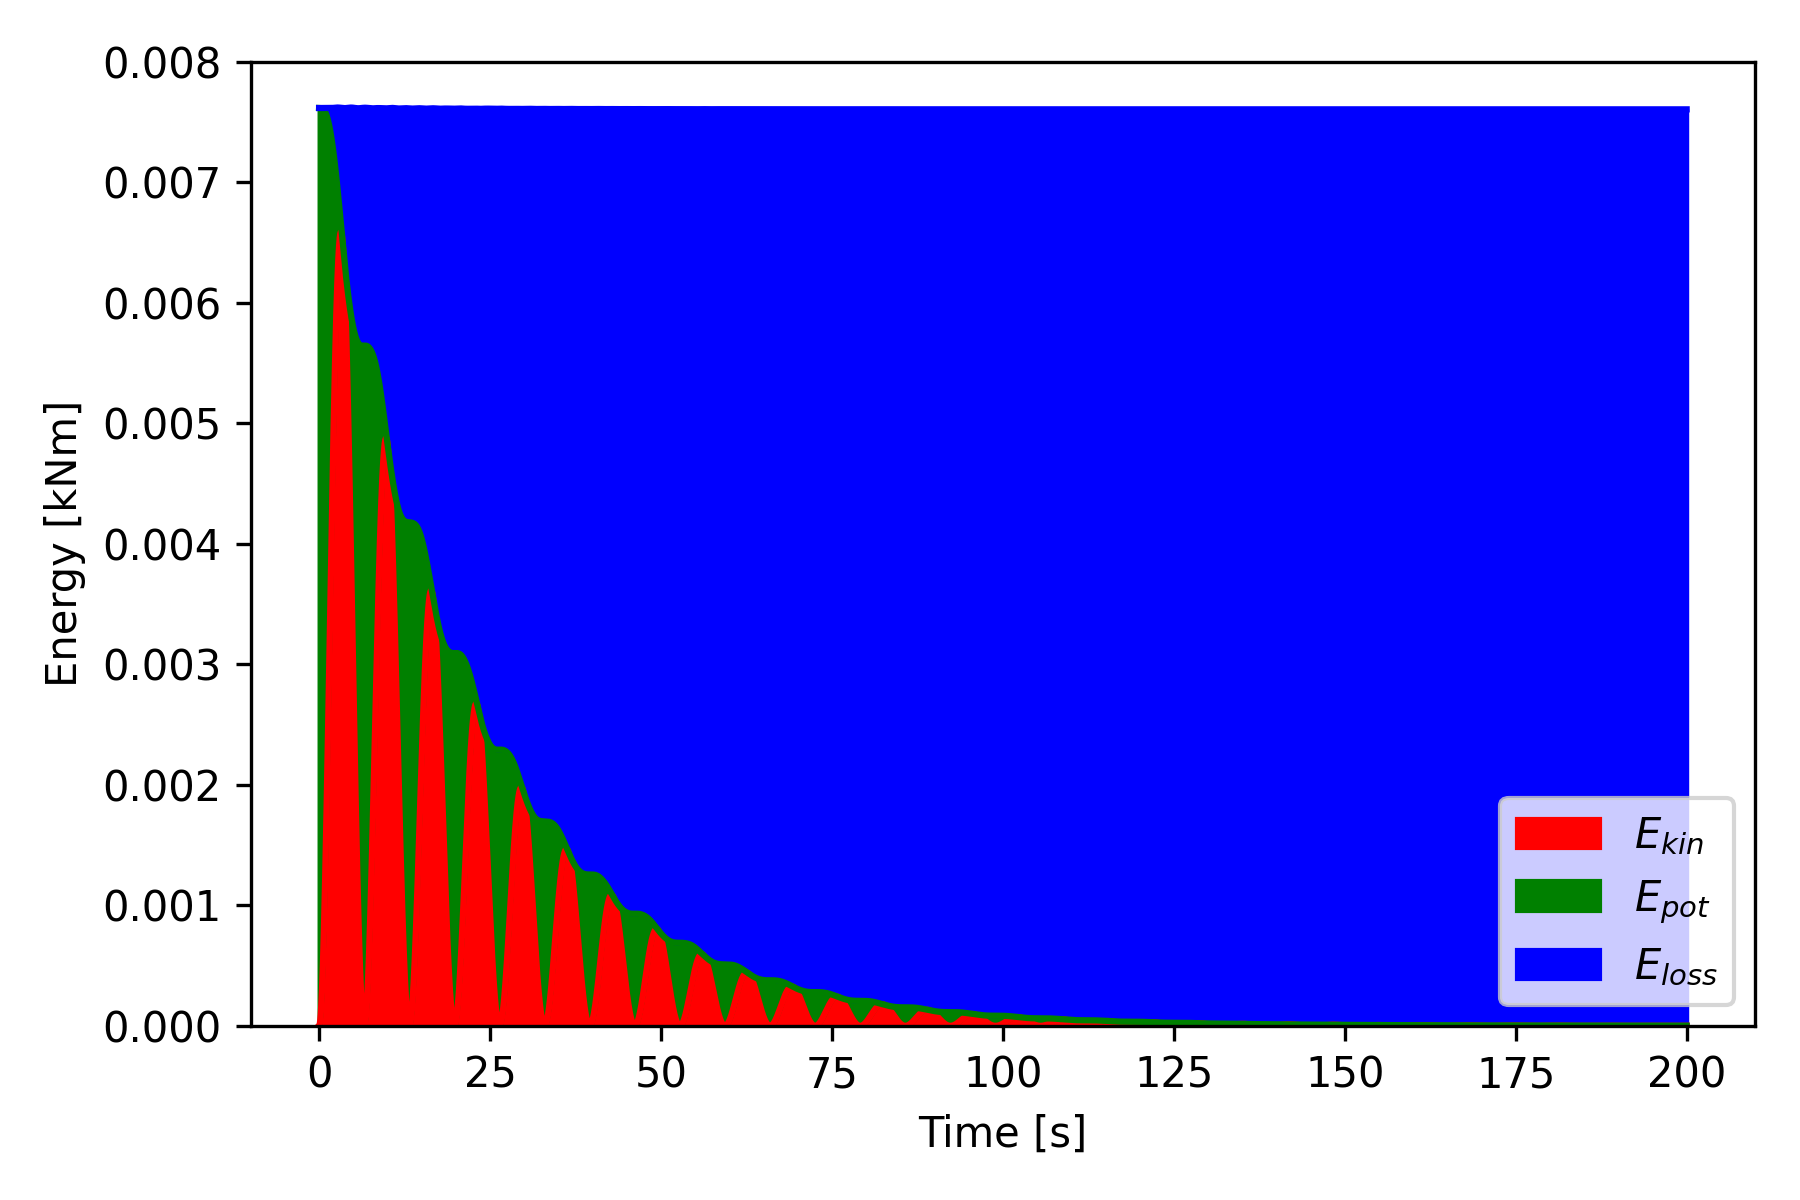
\includegraphics[width = 0.4\textwidth]{figures/energy.png}\end{center}
        \vspace{-1cm}
        \caption{Energy transfer}
        \label{fig:energy}
    \end{figure}

The linearized equivalent damping method is often treated as the best way to convert $B_1$, $B_2$, $B_3$ to frequency domain. Therefore, the most general way to determine the linear equivalent roll damping $B_e$ is to assume that the energy loss due to damping during a half cycle of roll is the same when nonlinear and linear damping are used \cite{7505983/RYUBZITQ}. Then $B_e$ can be calculated as a Fourier series expansion of the damping model as a cubic model:
    
\begin{equation}\label{eq:be_cubic}
B_{e} = B_{1} + \frac{8 B_{2} \omega_{0} \phi_{a}}{3 \pi} + 0.75 B_{3} \omega_{0}^{2} \phi_{a}^{2}.
\end{equation}

The expression above gives a relation between the frequency domain quantities $\phi_a$, $\omega_0$ and the time domain quantities $B_1$, $B_2$ and $B_3$ as in Eq.\eqref{eq:cubicroll}. In the case of a quadratic model $B_3=0$ and for the linear model $B_1$ and $B_e=B_1$ in Eq.\eqref{eq:be_cubic}.

\subsection*{Damping estimation by PIT from roll decay test} \label{subsec:damping_estimation}
When motion signals from either free roll decay model test or time domain numerical simulations, the parameters in the roll motion model Eq.\eqref{eq:rollmodel} can be identified using least square fit, since the time signals $\phi(t)$, $\dot{\phi}(t)$ and $\ddot{\phi}(t)$ can be calculated from the motion signal $\phi$. A parameters identification technique (PIT) similar to \cite{7505983/EXYJELCU} is used to obtain the damping coefficients from the roll decay model test as well as from the numerical simulated roll decay tests. In this technique, parameters in a mathematical model are determined in order to get the best fit to a roll decay time signal. \\


Alternatively, the other time derivatives can be estimated using numerical differentiation of a low-pass filtered roll signal or Kalman filtered roll signal. The filtering will however introduce some errors in itself. So instead of using this "Differentiation approach", it has been found that solving the differential equation numerically for guessed parameter values determined using optimization similarly to what was used by \cite{7505983/FJHQJJUH} and \cite{7505983/24TNAV5Z} gives the best parameter estimation. One problem with this "Integration approach" is that in order to converge, the optimization needs a reasonable first guess of the parameters. The Differentiation approach has therefore been used as a pre-step to obtain a very good first guess of the parameters that can be passed on to the Integration approach. This has been used for both signals from numerical and model tests.\\


In the following, the differential equation is numerically solved as an initial value problem. according to the example: $A_{44} = 1.0$, $B_1 = 0.3$, $C_1 = 5.0$. The initial states for $\phi(t)$, $\dot{\phi}(t)$ and $\ddot{\phi}(t)$ are used to estimate the following states, by
conducting very small time steps using the following expression for the acceleration. The analytical solution in Eq.\eqref{eq:analy_motion}, \eqref{eq:omega_zeta} and the numerical solution in Eq.\eqref{eq:cubicroll} are very similar as shown in Fig.(\ref{fig:analytical_numerical}). It also confirms that 

    \begin{figure}[t]
        \begin{center}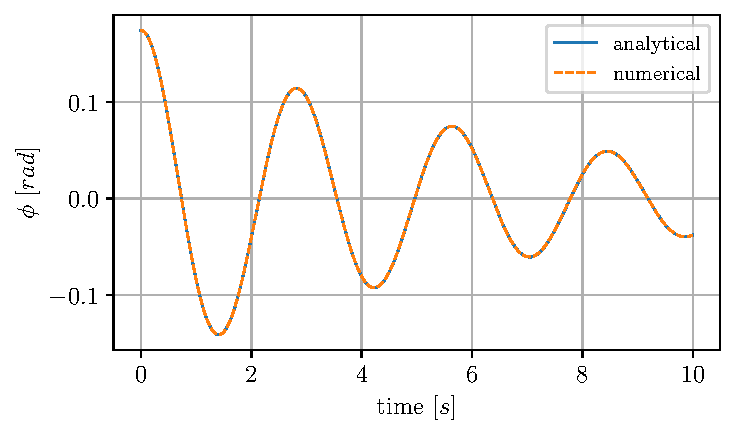
\includegraphics[width = 0.4\textwidth]{figures/analytical_numerical.pdf}\end{center}
        \vspace{-1cm}
        \caption{Analytical and numerical}
        \label{fig:analytical_numerical}
    \end{figure}

\subsection*{Ikeda's method for damping estimation} 
\label{subsec:damping_ikeda}

Alternatively, a well-recognized method for the damping estimation was developed by \cite{7505983/FB64RGPF}, also known as the Ikeda's method. It is defined in the frequency domain as in Eq.(\ref{eq:be_cubic}). In Ikeda's method, the equivalent linear damping $B_e$ can be estimated by the above PIT method based on large amount of roll decay tests. For the free roll decay tests, the coefficients in Eq.(\ref{eq:be_cubic}) $B_1$, $B_2$ and $B_3$ can be fitted by different initial roll decay amplitudes, while in this study the frequency $\omega$ is limited to the natural frequency of free roll decay tests $\omega_0$.  According to large amount of roll decay tests, Ikeda's method categorizes roll damping into five damping coefficients as in Table \ref{tab:damping_components}.\\

\begin{table}[ht]
\centering
\vspace{-0.5cm}
\caption{Damping components in Ikeda's method \label{tab:damping_components}}
\vspace{-0.2cm}
\begin{longtable}[]{@{}ll@{}}
\toprule
Symbol & Component\tabularnewline
\midrule
\endhead
$B_F$ & skin friction\tabularnewline
$B_E$ & eddy generation\tabularnewline
$B_L$ & hull lift\tabularnewline
$B_W$ & roll wave generation\tabularnewline
$B_{BK}$ & bilge keels\tabularnewline
\bottomrule
\end{longtable}
\end{table}

Then, the equivalent damping in Ikeda's method can be written as,


\begin{equation}
    B^{Ikeda}(\phi_a, \omega_0) = B_F + B_E + B_L + B_W + B_{BK},
\end{equation}

where the free roll decay tests are carrried out with initial roll amplitude $\phi_a$ with the natural roll frequency $\omega_0$.
Ikeda's method proposes semi-empirical formulas for the viscous damping components: $B_F$, $B_E$, $B_{BK}$ and $B_L$ so that viscous damping can be obtained from,

\begin{equation}
\label{eq:viscous damping}
B_{visc} = B_F + B_E + B_L + B_{BK}
\end{equation}

The linear and quadratic part of the viscous damping is obtained using the the equivalent linear damping method. In the case study KVLCC2 ship to validate our proposed method for roll damping estimation, due to the absence of bilge keels for the KVLCC2 the $B_{BK}$ does not need to be included in the viscous damping, other remaining components will get all the attention in this paper. \\

A schematic graph of how the parameters vary with speed and roll angle amplitude $\phi_a$ in the current model scale is created with the current implementation of Ikeda as shown below. The roll amplitude is first varied at zero speed (left). The speed is then varied from zero to the froude number corresponding to 15.5 knots in full scale for the KVLCC2 with a roll angle amplitude of 10 degrees (middle). The amplitude is then gradually reduced at the highest froude number down to zero again (right).
\pagebreak

\begin{figure}[H]
    \begin{center}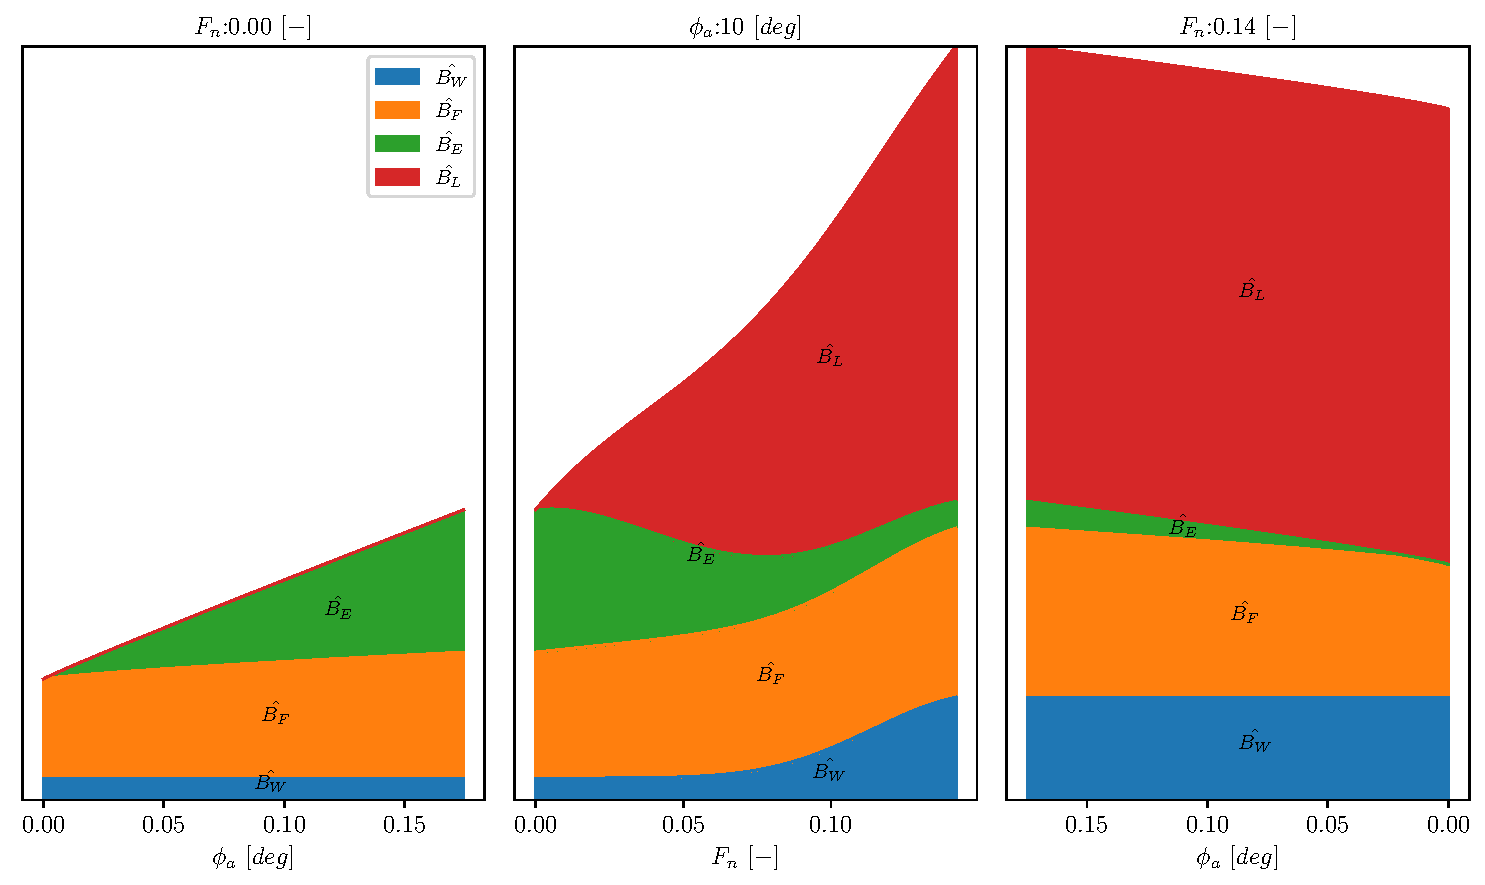
\includegraphics[width = 0.4\textwidth]{figures/ikeda_generic.pdf}\end{center}
    \vspace{-1cm}
    \caption{Ikeda generic}
    \label{fig:ikeda_generic}
\end{figure}

Assuming that the trends are correct in Ikeda's method it can be noted from the amplitude variations at zero knots (left):
\begin{itemize}
\item $B_W$ does not change with amplitude, implying that they only contribute to the linear part ($B_1$) of the damping. (The $B_W$ was calculated with strip theory here)
\item $B_F$ has a small amplitude dependency but the linear part is dominating.
\item $B_E$ has a large amplitude dependency and only contributes to the quadratic damping ($B_2$)\cite{7505983/4AFVVGNT}.
\end{itemize}

Looking at the speed variation (middle):

\begin{itemize}
\item At low speed $B_F$ and $B_E$ are the dominating components. (Note that this ship does not have bilge keels, as that would otherwise also be a large component).
\item At high speed the $B_E$ has almost disappeared and is replaced by the $B_L$ which is now the dominating component.
\item $B_F$ has a large contribution for all speeds (at model scale).
\end{itemize}

Looking at the roll amplitude variation (right):

\begin{itemize}
\item (Please note that this x-axis is revered in this graph)
\item $B_L$ does not change with amplitude, implying that they only contribute to the linear part ($B_1$) of the damping.
\item $B_F$ has a small amplitude dependancy but the linear part is dominating.
\end{itemize}

    
